\begin{figure*}[t]
\centering
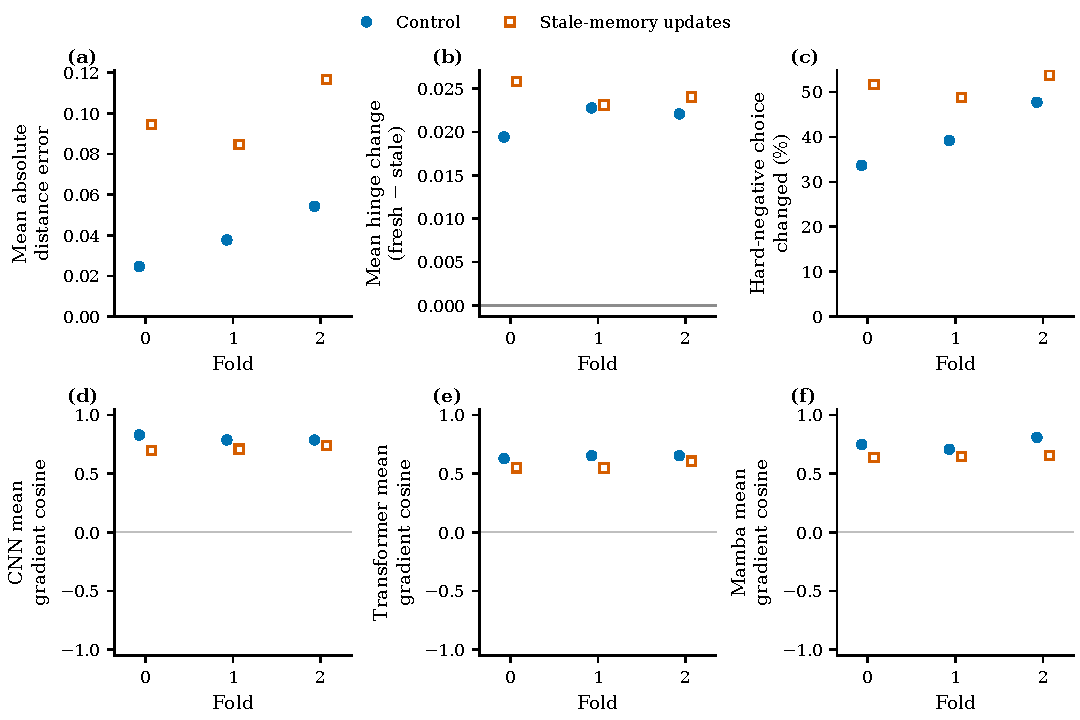
\includegraphics[width=\textwidth]{msvr310_freshness_preflight.pdf}
\caption{Complete short preflight only: six endpoints, 12 updates per endpoint, two warmup updates, one first-cache-fill update, and nine updates with historical candidates; full learning rate. This is a rendering and diagnostic check, not a full-source training trend. Control and stale-memory labels identify the actual training update rule; within each trajectory the same anchors, historical records, augmented views and current parameters are compared using cached versus freshly re-encoded historical coordinates. Fresh-coordinate losses never update the model. The compared metric term uses within-batch candidates for Control updates and cached expanded candidates for stale-memory updates; other training losses are unchanged. (a) Pair-weighted absolute difference of Euclidean distances between unit-normalized fused features for anchor--historical-candidate pairs only (64 times the historical candidate exposures). (b) Mean fresh minus stale batch-hard hinge loss. (c) Changed hard-negative selections divided by 64 times the number of updates with history. (d–f) Update-wise mean cosine between runtime-measured diagnostic gradients of the stale and fresh expanded losses on the same role encoder parameter block. Current peers retain gradients; historical candidates are detached in both comparisons. Gradient witnesses are runtime measurements, not independent CPU gradient recomputations. No-history metrics and undefined cosines are omitted, never set to zero. Folds are shown individually, without confidence intervals or a pooled-fold mean. These are source diagnostics, not held-out retrieval results. Historical update counts (control / stale-memory) for folds 0, 1, 2: 9 / 9; 9 / 9; 9 / 9. Undefined gradient cosine counts (CNN / Transformer / Mamba): 0 / 0 / 0.}
\label{fig:msvr310_freshness_preflight}
\end{figure*}
